% !TEX root = ../Hamiltonian_of_mean_force.tex
\section{Physical regimes of the mean-force state}
\label{sec:physical_regimes}
Even in this simple case, the physics encoded in the mean force state by its dependence on temperature and bath coupling is startlingly rich. To expose this, we first commit to a specific bath spectral density for numerics.  We choose
the Ohmic spectral density
\begin{equation}
  J(\omega) = \alpha\,\omega\,e^{-\omega/\omega_c},
  \qquad \omega\in[0,2\omega_q],
  \label{eq:J_ohmic}
\end{equation}
with $\alpha=1$ and $\omega_c = 5\omega_q$. Unless otherwise stated, we further specialise to $\theta=\pi/4$
throughout.  We emphasise here that the choice of spectral shape is not fundamental,
as it only controls the way in which $\chi$ runs
with temperature. 

This apparently innocuous expression encodes the entire non-perturbative recombination of bare Hamiltonian and influence, and functions as an \emph{order} parameter for the crossover between weak and strong coupling regimes. The reduced equilibrium state transitions between these regimes as $\chi$ passes through unity,
\begin{equation}
    \chi(\beta,g,\theta)\sim 1
    \qquad \Longleftrightarrow \qquad
    g^2 \sim \chi_0(\beta,\theta)^{-1}.
    \label{eq:chi_crossover_condition_v5}
\end{equation}



This crossover condition $\chi(\beta,g,\theta)=1$ therefore
defines a coupling-dependent temperature scale
\begin{equation}
  g_\star(\beta) = \chi_0(\beta,\theta)^{-1/2},
  \label{eq:gstar_def_v6}
\end{equation}
and an equivalent crossover temperature $\beta_\star(g)$. Notably, these dual crossover values are an exact property of the solution.

The function $\gamma(\chi)$ is elementary but worth dwelling on. It is monotone decreasing
from $\gamma(0)=1$ to $\gamma(\infty)=0$ with its inflection near $\chi\approx
1.2$, and admits clean asymptotic forms:
\begin{align}
  \chi \ll 1:\quad &\gamma \simeq 1 - \tfrac{\chi^2}{3}
    \quad\text{(weak coupling)},  \label{eq:gamma_weak}\\
  \chi \gg 1:\quad &\gamma \simeq \chi^{-1} = (g^2\chi_0)^{-1}
    \quad\text{(ultrastrong)}.   \label{eq:gamma_strong}
\end{align}
In the weak-coupling regime the state tracks the bare Gibbs thermal state with
$O(g^2)$ corrections, as expected. Notably, as shown in Fig.~\ref{fig:chi_theory}, the crossover between regimes depends on \emph{both} temperature and coupling strength. This means that two distinct regimes emerge in the limit of scaling $g$ and $\beta$, wholly dependent on which side of the crossover is taken. 

Notably, these critical temperatures and couplings have an \emph{involutive} relationship, in the sense that
\begin{equation}
    \beta_\star(g_\star(\beta)) = \beta, \quad g_\star(\beta_\star(g)) = g.
    \label{eq:involutive_relationship}
\end{equation}
This relationship between temperature and coupling means the crossover can be interpreted as the \emph{self-dual} line in the $(\beta, g)$ plane, as explored in Fig.~\ref{fig:involutive_map}. This line represents a coupling-dependent temperature scale $\beta_\star(g)$ (or equivalently $g_\star(\beta)$), where different parameter scaling relationships apply.

\begin{figure}[t]
  \centering
  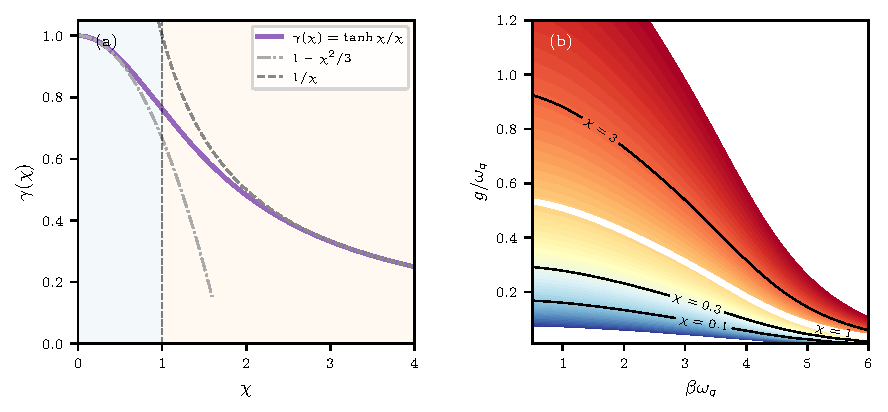
\includegraphics[width=0.48\textwidth]{../figures/hmf_fig1_chi_theory_ab.pdf}
  \caption{Universal crossover for the qubit mean-force state.
    \textbf{(a)} Crossover function $\gamma(\chi)=\tanh\chi/\chi$ interpolating
    between the weak-coupling approximant $1-\chi^2/3$ and the ultrastrong form
    $1/\chi$.  Shaded regions mark the weak (blue) and strong (orange) regimes
    separated by $\chi=1$.
    \textbf{(b)} Dimensionless coupling $\chi(\beta,g) = g^2\chi_0(\beta)$ as a
    contour map.  Vertical trajectories (fixed $g$) will crossover at its corresponding
    $\beta_\star(g)$.}
  \label{fig:chi_theory}
\end{figure}

\begin{figure}[t]
    \centering
    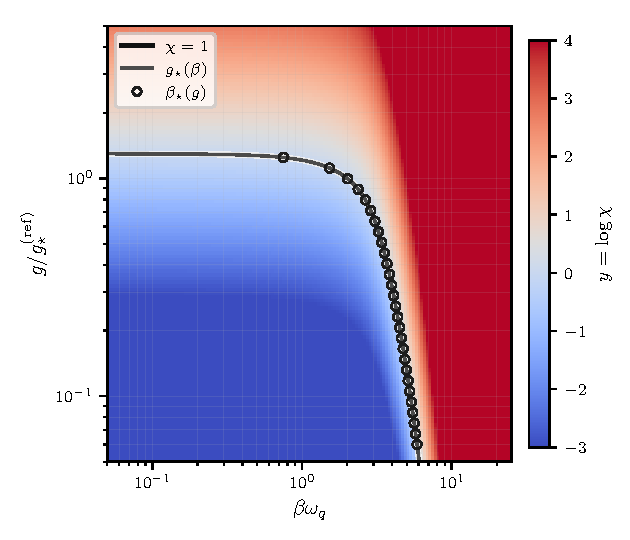
\includegraphics[width=0.48\textwidth]{../figures/hmf_crossover_involutive_v1.pdf}
    \caption{Involutive crossover geometry generated by $\chi(\beta,g) = g^2\chi_0(\beta)$. 
    The heatmap shows $y = \log\chi$ in the $(\beta, g)$ plane. The solid black line marks the crossover locus $\chi=1$, which can be constructed either as a coupling-dependent temperature $\beta_\star(g)$ (circles) or a 
    temperature-dependent coupling $g_\star(\beta)$ (solid grey line). This involutive relationship defines a partition between the weak-coupling (blue) and strong-coupling (red) scaling regimes.}
    \label{fig:involutive_map}
\end{figure}

\subsection{State purity}
\label{subsec:purity}
The purity of the qubit mean-force state is $\mathcal{P} = \tfrac{1}{2}(1 +
r^2)$ with $r^2 = |\mathbf{r}|^2$. From this we can immediately establish a universal result:

\begin{quote}
\textbf{Bath always purifies.}\; \textit{For any positive spectral density
$J(\omega)\geq 0$ and any $\beta>0$: (i) $r^2(g,\beta)$ is strictly increasing
in $g$ for $g\geq 0$, and (ii) for all $g>0$,}
\begin{equation}
    r^2(g,\beta) \;>\; r_{\rm bare}^2 \;\equiv\; \tanh^2\!\left(\frac{\beta\omega_q}{2}\right),
    \label{eq:purity_bound}
\end{equation}
\textit{with equality only at $g=0$.}
\end{quote}

\paragraph{Proof sketch.}
Part~(i) (monotonicity) follows immediately from the exact formula $r =
\tanh\chi = \tanh(g^2\chi_0(\beta))$: since $\tanh$ is strictly increasing and
$g^2\chi_0$ is strictly increasing in $g$, so is $r$.

Part~(ii) (excess over bare) uses the non-negativity of the resonant (longitudinal) dressing $\Sigma_z$. From the explicit integral form of the response kernels (cf.\ App.~\ref{app:qubit_ladder_derivation}), one has
\begin{equation}
    \Sigma_z = \frac{1}{\pi}\int_0^\beta u(\beta-u)\,K(u)\,\frac{\sinh(\omega_q u)}{u}\,du.
\end{equation}
Since $K(u)\geq 0$ for a physical spectral density, and the remaining factors are non-negative on the integration domain, we have $\Sigma_z > 0$ for all $\beta>0$. 

Substituting the exact components $m_z = \tanh \Theta$ and $m_\perp$ from Eq.~\eqref{eq:bloch_locking_linear}, the purity excess $\Delta r^2 = r^2 - \tanh^2(\beta\omega_q/2)$ is found to be strictly positive whenever $\gamma s^2 \Sigma_z > 0$. Physically, this reflects the fact that the bath-induced longitudinal field always reinforces the system's tendency to polarise, effectively lowering the local temperature and thus increasing the purity of the state beyond its bare thermal value. $\square$

In the limit $\beta\to 0$ (infinite temperature), the bare state is maximally mixed, yet the
mean-force state has
\begin{equation}
    r\big|_{\beta\omega_q\to 0} = \tanh\chi > 0,
    \label{eq:purity_highT}
\end{equation}
This result is independent of the bandwidth or spectral shape of $J(\omega)$:
widening the bath increases $\chi_0(\beta)$ (driving the crossover to weaker
$g$) but cannot reverse the purity inequality.  Purity inversion would require
reversing the sign of the longitudinal response ($\Sigma_z < 0$), which is impossible for
any physical (positive) spectral density. 

Figure~\ref{fig:purity_figure} confirms this numerically. Panel (a) shows $r(g/g_\star)$ for four temperatures.
Every trajectory lies strictly above its own $r_{\rm bare}$ reference line for
all $g>0$, confirming~\eqref{eq:purity_bound}. Panel (b) shows the purity excess $\Delta r^2 = r^2 -
\tanh^2(\beta\omega_q/2)$ over the full $(g,\beta)$ plane.  Enhancement peaks at large $g$
and high temperature (upper-right corner), and falls to near zero at low
temperature (left edge) where the bare state is already nearly pure.  The black dashed contour $\chi=1$ marks the crossover at which purification
accelerates steeply. This is an amusingly counterintuitive result - for sufficiently strong coupling, a \emph{hotter} bath is \emph{more} purifiying!

Finally, we note that there is a slight tension in this result when compared to the renormalised perspective. In particular, from Eq.~\eqref{eq:bloch_locking_linear}, where we associate the state radius with an effective inverse temperature $\tilde{\beta} = 2\chi/\omega_q$, a purity decrease would require $\tilde{\beta}$ to fall below its bare value. Should the effective temperature ever cross into the negative regime, this would correspond to a \emph{population inversion} in the renormalised system. However, since the coupling $g$ is measured in inverse units of $\omega_q$, the resonant reinforcement $\Sigma_z$ scales such that for any \emph{finite} coupling and splitting, the influence parameter $\chi = g^2\chi_0$ is strictly positive. This ensures that the effective inverse temperature $\tilde{\beta}$ remains strictly positive and bounded from below by its bare thermal value for all $g>0$. Thus, for any physical bath, no finite coupling can ever induce a population inversion, confirming that the bath serves only to order and purify the qubit state.

\begin{figure}[t]
    \centering
    
\includegraphics[width=\columnwidth]{../figures/hmf_purity_figure.pdf}
    \caption{Purity of the qubit mean-force state.
    \textbf{(a)} Bloch radius $r$ versus scaled coupling $g/g_\star(\beta)$
    for four temperatures.  Dotted horizontals show the bare thermal purity
    $r_{\rm bare} = \tanh(\beta\omega_q/2)$; coupling always increases purity
    (Eq.~\eqref{eq:purity_bound}), most visibly at high temperature where the
    bare state is near-maximally-mixed.  Shaded regions mark the weak (blue) and
    strong (orange) coupling regimes.
    \textbf{(b)} Purity excess $\Delta r^2 = r^2 - \tanh^2(\beta\omega_q/2)$ in the
    $(g,\beta)$ plane.  The black dashed contour marks the crossover locus
    $\chi=1$: purification is strongest at large $g$ and high temperature and
    saturates as $r\to 1$ deep in the strong-coupling regime.}
    \label{fig:purity_figure}
\end{figure}

\begin{figure}[t]
    \centering
    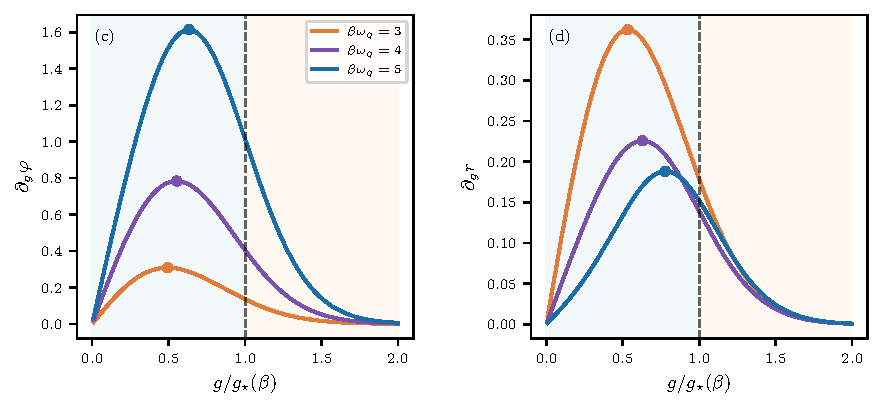
\includegraphics[width=0.48\textwidth]{../figures/hmf_fig1_chi_theory_cd.pdf}
    \caption{Coherence and purity susceptibilities.
    \textbf{(c)} Bloch-angle susceptibility $\partial_g\varphi$ versus scaled
    coupling $g/g_\star(\beta)$ for three temperatures.  Rescaling collapses the
    peak positions to a universal value $g/g_\star \approx 0.65$, marked by filled
    circles.
    \textbf{(d)} Purity gradient $\partial_g r$; the rescaled peak occurs at
    $g/g_\star \approx 0.92$.}
    \label{fig:chi_susceptibility}
\end{figure}

\subsection{Quantum Enhancement of Heat Engines}
An interesting feature of the crossover regime is that it demarcates the region where the state is maximally sensitive to bath coupling. This is easily seen by considering the susceptibilities of the tilt angle $\partial_g\varphi$ and Bloch radius $\partial_g r$. These quantify how rapidly the Bloch vector tilts and how rapidly the state purifies per unit change in $g$. As Fig.~\ref{fig:chi_susceptibility} shows, both peak near the
crossover $\chi =1$. $\partial_g\varphi$ maximises at $g \approx 0.65\,g_\star$
(at $\chi_{\rm peak,\varphi}\approx 0.42$) and $\partial_g r$ maximises at $g
\approx 0.92\,g_\star$ ($\chi_{\rm peak,r}\approx 0.85$).  The locations are
approximately pinned at universal values of $\chi$ independent of temperature, as demonstrated by the alignment of peaks when plotted as a function of the rescaled coupling $g/g_\star(\beta)$. The crossover region $\chi\sim 1$ is therefore where bath coupling yields the
greatest rate of return: both the onset of coherence (tilt of the Bloch vector
away from the bare thermal axis) and the onset of purification are most rapid
here, before both effects saturate as $\chi\to\infty$.  This suggests the
crossover regime is the most operationally leveragable for state engineering. 

We can immediately demonstrate this phenomenon with a toy model of a heat engine. In particular, we consider an Otto-stroke cycle, with unitary strokes. This can extract at most the system
\emph{ergotropy} per stroke with respect to the stroke Hamiltonian. The ergotropy of a state $\rho$ with respect to $H_Q$ is

\begin{equation}
  W_{\rm erg}(\rho,H_Q)
  = \Tr(\rho H_Q) - \min_{U}\Tr(U\rho U^\dagger H_Q),
  \label{eq:ergotropy_def}
\end{equation}

where the minimisation is over all unitaries $U$.  For any qubit the
minimiser is a \emph{passive rearrangement}. The Bloch vector is simply rotated
antiparallel to the ground direction $-\hat{\mathbf{n}}_s$ of $H_Q$ at
fixed spectrum.  The passive state has Bloch vector $\vec{m}^{\,\rm pas}
= -r\hat{\mathbf{n}}_s$ and energy $-\omega_q r/2$.  

The astute reader may already have noticed that the renormalised perspective already contains within it an implicit quantum advantage, but for the slower thinkers we shall make it explicit. The argument proceeds in two steps. We first define the quantum advantage over an incoherent cycle by the \emph{coherence-enabled ergotropy}. Letting $\delta[\rho]\equiv\operatorname{diag}(\rho)$
denote the dephased state in the $H_Q$ eigenbasis. From this, the coherent contribution to ergotropy is simply:
\begin{equation}
\begin{split}
  \delta W_{\rm coh} &:= W_{\rm erg}(\rho,H_Q) - W_{\rm erg}(\delta[\rho],H_Q) \\
  &= \frac{\omega_q}{2}\!\left(\sqrt{m_z^2+m_\perp^2}+m_z\right), \qquad m_z\leq 0,
\end{split}
\label{eq:delta_W_coh}
\end{equation}

Both equalities in Eq.~\eqref{eq:delta_W_coh} warrant justification.
The physics decomposes cleanly into two independent structural facts. First, \emph{the dephased state is always passive}. Energy dephasing leaves a diagonal state $\delta[\rho]$ with populations
$p_\pm = (1\pm m_z)/2$.  For $\delta[\rho]$ to be passive one needs the
larger eigenvalue on the lower-energy level, i.e.\ $p_- \geq p_+$, which
reduces to $m_z \leq 0$.  This is guaranteed by the bath: $\Sigma_z > 0$
for any positive spectral density (established in Sec.~\ref{subsec:purity}),
which forces $m_z < 0$ at all finite $g$ and $\beta$.  An incoherent cycle
running on $\delta[\rho]$ therefore extracts zero work,
$W_{\rm erg}(\delta[\rho],H_Q)=0$, and the first equality in
Eq.~\eqref{eq:delta_W_coh} reduces to
$\delta W_{\rm coh} = W_{\rm erg}(\rho,H_Q)$.

The second crucial fact is that for any $\theta \neq 0, \pi/2$, the bath tilts the Bloch vector away from the passive direction $-\hat{\mathbf{n}}_s$ through the anisotropy
$\tan\eta=-\cot\theta\,\Sigma_\perp/\Sigma_z$
(Eq.~\eqref{eq:theta_eta_params}), generating a non-zero transverse
magnetisation $\tilde{m}_\perp\propto\Sigma_\perp$
(Eq.~\eqref{eq:effective_magnetisations}). Then one has $m_\perp\neq 0$ and thus
$r > |m_z|$.  The ergotropy of the mean-force state is then
\begin{equation}
  W_{\rm erg}(\rho,H_Q) = \frac{\omega_q}{2}(r + m_z) > 0,
  \label{eq:ergotropy_qubit}
\end{equation}
with the exact solution $r=\tanh\chi$, $m_z=\tanh\Theta$ giving the
closed form
\begin{equation}
  W_{\rm erg} = \frac{\omega_q}{2}(\tanh\chi + \tanh\Theta).
  \label{eq:ergotropy_exact}
\end{equation}

These facts in combination establish quantum advantage as a structural guarantee: $\delta W_{\rm coh}>0$ for any physical
broadband bath, independently of coupling strength or temperature.It does
not of course guarantee positive \emph{net} work output from a complete cycle. This will depend on the control cost
of modulating the coupling $g$, which generates and maintains the
transverse coherence $m_\perp$. Nevertheless, we may use these results to establish that the ergotropy gain is maximised in the crossover regime $\chi \sim 1$. 

Differentiating Eq.~\eqref{eq:ergotropy_qubit} with respect to coupling,
\begin{equation}
  \partial_g W_{\rm erg} = \frac{\omega_q}{2}(\partial_g r + \partial_g m_z),
  \label{eq:dWerg_dg}
\end{equation}
both terms receive contributions from the purity susceptibility $\partial_g r$
and the tilt susceptibility $\partial_g\varphi$ that peak in the crossover
band $\chi \sim 1$ (Fig.~\ref{fig:chi_susceptibility}).  The ergotropy
gradient therefore also peaks within this band. The crossover regime
$\chi \sim 1$ is where coupling most efficiently converts bath influence
into extractable work.  Figure~\ref{fig:ergotropy} shows this directly: the susceptibility
$\partial_g W_{\rm erg}$ peaks near $g\approx g_\star$ at a value that
grows monotonically with $\beta$, while $\delta W_{\rm coh}$ itself
turns on at the crossover and saturates at a $\beta$-dependent level.
The crossover is therefore the operational marker for engine-relevant
resource generation, and the effect is amplified at lower temperatures
where the transverse bath channel $\Sigma_\perp$ becomes dominant. This translates into a general design principle for quantum engines - that their efficiency is maximised when the coupling is modulated around the crossover band. 

\begin{figure}[t]
  \centering
  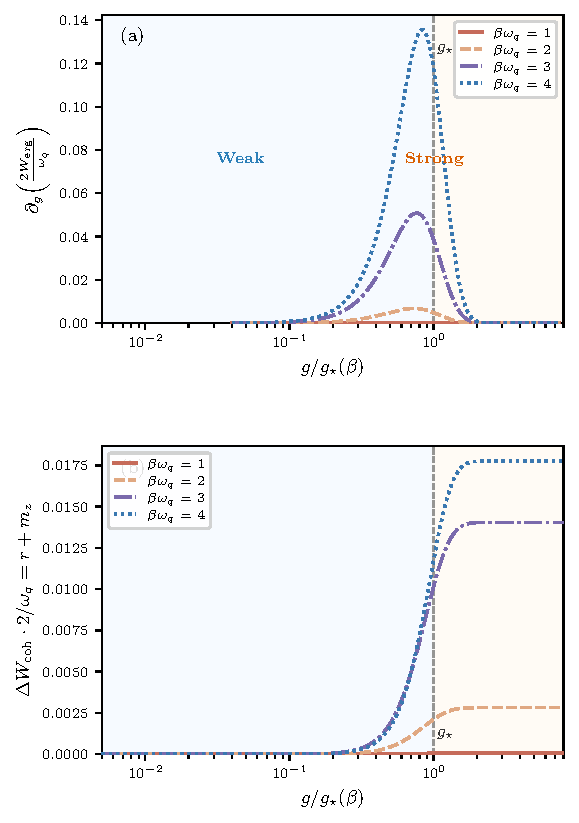
\includegraphics[width=\columnwidth]{../figures/hmf_ergotropy.pdf}
  \caption{Coherence-enabled ergotropy of the qubit mean-force state.
    \textbf{(a)} Ergotropy susceptibility
    $\partial_g \delta W_{\rm coh}$ versus $g/g_\star(\beta)$.
    The peak position locks near the crossover $g\approx g_\star$
    independent of temperature, while the peak height increases
    monotonically with $\beta$: low temperatures activate the
    transverse bath channel and make coherence-enabled work extraction
    increasingly efficient.
    \textbf{(b)} Coherence-enabled ergotropy
    $\delta W_{\rm coh}$ versus $g/g_\star(\beta)$ (calculated for $\omega_q=1$).  Since $m_z<0$ throughout,
    $W_{\rm erg}(\delta[\rho])=0$ and $\delta W_{\rm coh}=W_{\rm erg}$
    (Proposition~\ref{prop:coh_erg}).  The onset occurs at the
    crossover and the saturation value grows with $\beta$,
    reflecting the increasing importance of the transverse bath
    channel $\Sigma_\perp$ at lower temperatures.}
  \label{fig:ergotropy}
\end{figure}

There is a final irony to this result.  While being most expolitable, this regime is simultaneously the most demanding for
numerical simulation.  Exact Diagonalisation (ED) of the truncated spin-boson
model faces two convergence requirements that become simultaneously binding
near $\chi\sim 1$.  On the spectral side, a faithful discretisation of $J(\omega)$
requires a mode count $N_\omega$ large enough to accurately quadrature the bath
kernel at $\omega\in\{0,\pm\omega_q\}$: at the crossover these integrals receive
comparable contributions from the full spectral window, so neither the infrared
nor the ultraviolet modes can be coarsened without systematic bias.  On the
state-space side, representing the polaron-like mean-force ground state demands
a per-mode Fock cutoff $n_{\max}\gtrsim\alpha_k^2$, where the mode displacement
$\alpha_k = g\,c_k/\omega_k$ is already appreciable at $g\sim g_\star(\beta)$
yet the state has not saturated to the simple displaced-vacuum structure it
acquires only at $\chi\gg 1$.  Neither the weak-coupling approximation nor the
ultrastrong polaron limit simplifies the representation, so both hierarchies
must be converged together.  The $\chi=1$ crossover partitions parameter
space into an ED-reliable sector ($\chi\lesssim 1$) and a
polaron-representability-limited sector ($\chi\gtrsim 1$), with the
susceptibility peaks sitting squarely on this boundary. 

 
\subsection{Temperature-driven and coupling-driven limits}
\label{subsec:limits}
We now turn our attention to two\footnote{There is a third limit, but it lies outside the present scope of our discussion} of the limiting cases of the qubit mean-force state: the coupling-driven limit ($g\to\infty$ at fixed $T$) and the temperature-driven limit ($T\to 0$ at fixed $g$). The first observation is that $g\to\infty$ at fixed $T$ and $T\to 0$ at fixed $g$ drive $\chi\to\infty$
and hence $r\to 1$.  Yet the two limits land at entirely different points on the
Bloch disk boundary.  The state's location is set by two bath-dependent
quantities: the tilt-angle parameter $\eta$ [Eq.~\eqref{eq:theta_eta_params}]
and the effective-temperature shift $\Theta+\beta\omega_q/2 =
\operatorname{arctanh}(\gamma s^2\Sigma_z)$.  In both limits $\gamma\to 0$, but
the product $\gamma s^2\Sigma_z$ behaves oppositely, and this is the root of
the distinction.

\begin{figure}[t!]
    \centering
    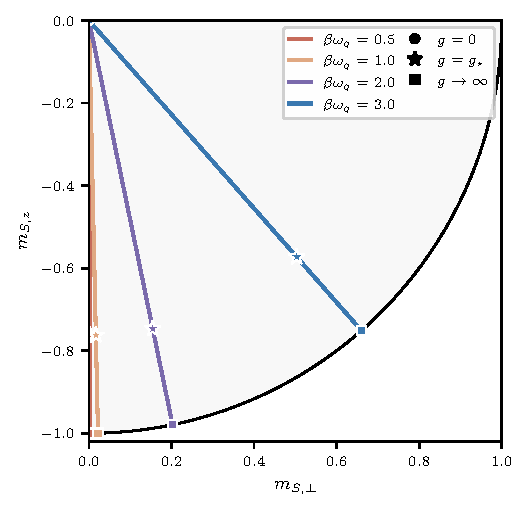
\includegraphics[width=0.8\columnwidth]{../figures/hmf_bloch_disk_portrait.pdf}
    \caption{Trajectories of the mean-force Bloch vector in the coupling plane.  Coordinates: longitudinal
    polarisation $m_z = \langle\sigma_z\rangle$ vs.\ transverse
    polarisation $m_\perp = \langle\sigma_\perp\rangle$, plotted on a square-root scale $\sqrt{m_\perp}$ to resolve the crossover region.  The dashed line marks
    the direction $\varphi$ of the strong-coupling attractor for the lowest temperature shown.
    \textbf{(a)} Coupling-driven trajectories: fixed $\beta\omega_q \in
    \{0.5,1.0,2.0,3.0\}$, coupling $g$ swept from $0$ to $\infty$.  Circles:
    bare thermal state ($g=0$).  Stars: crossover $g=g_\star$.  Squares:
    strong-coupling attractor ($g\to\infty$).  The squares lie at
    different positions for each $T$, demonstrating temperature memory.
    \textbf{(b)} Temperature-driven trajectories: fixed coupling values $g/\omega_q \in \{0.2, 0.5, 1.0, 2.0\}$
    swept over $\beta$. To eliminate the exponentially scaling DC component of the non-resonant bath influence, we assume a bath with a small IR cutoff frequency $\omega_{\rm min} = 0.04\omega_q$. Circles: $T\to\infty$.  Stars: $T=T_\star(g)$.
    Squares: $T\to 0$ (all converge to $-\hat{\mathbf n}_s$, the ground state).
    At large $g$ (top curves) the state traces near the disk boundary, a
    precession at near-unit purity as the attractor direction drifts with
    temperature.}
    \label{fig:bloch_disk_portrait}
\end{figure}

\paragraph{Coupling-driven limit: $g\to\infty$ at fixed $T$.}
Factoring out the coupling as $K(u)=g^2 K_0(u)$ shows that both bath channels
scale identically with $g$: $\Sigma_z = g^2\Sigma_z^{(0)}$ and
$\Sigma_\perp = g^2\Sigma_\perp^{(0)}$, so $\chi = g^2\chi_0(\beta)$.  
The key observation is that any ratio of bath-induced quantities is independent of $g$ in this limit.
More precisely, for any two observables $A(g), B(g)$ that each scale as $g^2$, an L'Hopital-style argument gives
\begin{equation}
  \lim_{g\to\infty} \frac{A(g)}{B(g)} = \lim_{g\to\infty} \frac{g^2 A^{(0)}}{g^2 B^{(0)}} = \frac{A^{(0)}}{B^{(0)}},
  \label{eq:ginfty_ratio}
\end{equation}
where $A^{(0)}, B^{(0)}$ are the $g$-independent amplitudes. Although individually
$\gamma=\tanh\chi/\chi\to 0$ and $\Sigma_z\to\infty$ as $g\to\infty$, their product is an example of this rule:
\begin{equation}
  \gamma s^2\Sigma_z = \frac{\tanh(g^2\chi_0)}{g^2\chi_0}\cdot g^2 s^2\Sigma_z^{(0)}
  \;\xrightarrow{g\to\infty}\; \frac{s^2\Sigma_z^{(0)}}{\chi_0(\beta)},
  \label{eq:ginfty_dressing}
\end{equation}
which is a finite, purely temperature-dependent quantity. Crucially, the tilt-angle ratio
$\Sigma_\perp/\Sigma_z = \Sigma_\perp^{(0)}/\Sigma_z^{(0)}$ is likewise $g$-independent.
The entire $g$-dependence of the trajectory therefore enters only through $\gamma(g^2\chi_0)$,
which controls how far along the trajectory --  from the bare state at $g=0$ to the
asymptotic attractor -- the state has been driven.  The attractor itself is a fixed
point in the $(m_\perp, m_z)$ plane whose location is set by $\beta$ alone and is
independent of how large $g$ is taken.  This is the \emph{temperature memory} of the
system: the strong-coupling attractors (squares in Fig.~\ref{fig:bloch_disk_portrait}(a))
label a $\beta$-parameterised curve on the disk boundary.

\paragraph{The crossover at $g_\star$ and the two regimes.}
The coupling scale $g_\star$ defined by $\chi(\beta,g_\star)=1$ [Eq.~\eqref{eq:chi_crossover_condition_v5}]
partitions the trajectory into two qualitatively distinct segments.  For $g<g_\star$
($\chi<1$), $\gamma>\tanh(1)\approx 0.76$ and the bath dressing is sub-critical: the
effective temperature $\tilde\beta$ remains close to the bare value and the state
stays well within the disk, close to the bare thermal state.  For $g>g_\star$
($\chi>1$), $\gamma$ drops rapidly and the state is driven strongly toward the
attractor: the purity $r=\tanh\chi$ saturates toward 1 and the effective temperature
departs significantly from bare $\beta$.  The star markers in panel~(a) mark the
bend in each trajectory — the onset of the bath-dominated regime — where the
state leaves the interior of the disk and begins hugging the boundary.  Notably,
for $g\gg g_\star$ the effective dressing $\gamma s^2\Sigma_z$ saturates to its
asymptotic value and the state freezes at the attractor, regardless of how much
further $g$ is increased.

\paragraph{Temperature dependence of the attractor and connection to the Cresser--Anders limit.}
The attractor location itself shifts with temperature.  From
Eqs.~\eqref{eq:ginfty_dressing} and~\eqref{eq:theta_eta_params}, the attractor
direction is governed by
$\tan\eta^{(\infty)} = -\cot\theta\,\Sigma_\perp^{(0)}/\Sigma_z^{(0)}$,
which grows with $\beta$ (since $\Sigma_\perp^{(0)}$ grows exponentially and
$\Sigma_z^{(0)}$ only linearly): as temperature decreases, the attractor drifts to
larger $m_\perp$, tracing a curve toward the coupling-axis direction $\pi-\theta$.
This drift is directly visible in panel~(a): the cold attractors (blue squares) lie
further from the pole than the hot ones (red squares).

This observation connects naturally to the ultrastrong limit studied by Cresser and
Anders~\cite{cresserWeakUltrastrongCoupling2021a}.  Their argument treats the bare
qubit Hamiltonian $H_Q$ as a perturbation on the joint system-bath in the limit
$g\to\infty$ -- in effect taking $g/\omega_q\to\infty$ so that the qubit frequency
becomes infinitesimal relative to the coupling scale.  From our perspective, this
corresponds to evaluating both bath channels in the $\omega_q\to 0$ limit, where
the frequency selectivity between $\Sigma_z$ and $\Sigma_\perp$ is lost and both
channels probe the same low-frequency spectral weight.  In that limit the ratio
$\Sigma_\perp/\Sigma_z$ diverges (since $\Sigma_z\propto\omega_q$ vanishes while
$\Sigma_\perp$ remains finite), driving $\tan\eta^{(\infty)}\to\infty$ and the
attractor to the direction of the coupling axis $\hat{\mathbf f}$, consistent with
the Cresser--Anders result.  Our temperature-resolved picture reveals that this
alignment with $\hat{\mathbf f}$ is the \emph{zero-temperature endpoint} of the
attractor drift: at any finite temperature the attractor sits at an intermediate
angle encoding the competition between $\omega_q$ and the bath-induced dressing.

\paragraph{Two $\beta\to\infty$ scenarios: DC bath versus IR gap.}
The $\Sigma_\perp/\Sigma_z$ ratio is the key object because it determines both $\eta$
(the attractor direction) and feeds into $\chi$ (which drives $r\to 1$).  Its
$\beta$-dependence is controlled by the bath's low-frequency spectral structure.
The longitudinal channel is \emph{universal}:
\begin{equation}
  \Sigma_z = \tfrac12[R(\omega_q)-R(-\omega_q)] \;\sim\; \beta\lambda, \qquad
  \lambda \equiv \int_0^\infty\frac{d\omega\,J(\omega)}{\omega},
  \label{eq:Sigma_z_linear}
\end{equation}
growing \emph{linearly} with $\beta$ for any bath with finite spectral weight at
$\omega_q$.  This reflects the linear growth of the detailed-balance asymmetry
$R(\omega) - R(-\omega) = 2\beta\omega\lambda$ with inverse temperature.  In contrast,
the non-resonant channel [Eq.~\eqref{eq:bath_kernels_direct}]
\begin{equation}
  \Sigma_\perp \approx \frac{4}{\omega_q}\Bigl[
    \cosh\!\left(\tfrac{\beta\omega_q}{2}\right)\mathcal{K}(0)
    - e^{-\beta\omega_q/2}\mathcal{K}(\omega_q)\Bigr]
  \label{eq:Sigma_perp_expanded}
\end{equation}
exhibits a qualitative bifurcation depending on the bath IR structure:

\begin{itemize}
  \item \textbf{DC bath} ($\omega_{\min}=0$, finite $\mathcal{K}(0)>0$): the
  $\cosh(\beta\omega_q/2)$ prefactor drives $\Sigma_\perp\propto e^{\beta\omega_q/2}$
  \emph{exponentially}, so $\Sigma_\perp/\Sigma_z \propto e^{\beta\omega_q/2}/\beta\to\infty$.
  Via Eq.~\eqref{eq:theta_eta_params}, $|\tan\eta|\to\infty$ and $\eta\to\pi/2$,
  precessing the state toward $\pi-\theta$.  Simultaneously $\chi\sim s|c|\Sigma_\perp$
  grows exponentially, so the crossover $\chi\sim 1$ occurs at a finite $\beta_\star$,
  after which the state rapidly saturates to a pure state at the coupling-axis attractor.

  \item \textbf{IR-gapped bath} ($\omega_{\min}>0$, so $\mathcal{K}(0)\to 0$ exponentially
  below $\omega_{\min}$): the DC term is quenched and the surviving term decays,
  $\Sigma_\perp\sim e^{-\beta\omega_q/2}$.  The ratio $\Sigma_\perp/\Sigma_z\to 0$,
  and $|\tan\eta|\to 0$: the effective field aligns with $\hat{\mathbf n}_s$ and the
  coherences are quenched.  With $\gamma s^2\Sigma_z \propto\Sigma_z/\Sigma_\perp\to 0$,
  the effective-temperature shift vanishes and $m_z\to -\tanh(\beta\omega_q/2)$.
  At this value the prefactor $m_z\cosh(\beta\omega_q/2)+\sinh(\beta\omega_q/2)$
  in Eq.~\eqref{eq:bloch_locking_linear} is exactly zero, so $m_\perp=0$ identically:
  the state collapses to the bare ground state $-\hat{\mathbf n}_s$.
\end{itemize}

This is why the two panels of Fig.~\ref{fig:bloch_disk_portrait} look so different:
panel~(a) (fixed $\beta$, $g$-sweep) operates at fixed $\Sigma_\perp/\Sigma_z$ and shows
trajectories converging to temperature-dependent attractors on the disk boundary;
panel~(b) (fixed $g$, $\beta$-sweep with $\omega_{\min}>0$) tracks the IR-gapped
scenario and all trajectories converge to the same south pole, even those that closely
approach the boundary at intermediate $\beta$.


\subsection{Relation to the Cresser--Anders ultrastrong limit}
\label{subsec:qubit_relation_to_limits}

It is instructive to make explicit how the exact qubit geometry relates to the
ultrastrong mean-force result of Cresser and Anders.  Their central statement
is a \emph{basis-selection} theorem: as the coupling scale $\lambda\to\infty$,
the mean-force Gibbs state becomes diagonal in the eigenbasis of the coupling
operator $X$ rather than in the bare Hamiltonian basis
$H_Q$~\cite{cresserWeakUltrastrongCoupling2021a}.  For a qubit with coupling
axis $\hat{\mathbf f}$ this yields a limiting Bloch vector pointing along
$\hat{\mathbf f}$ (with magnitude set by the projected bare splitting).  In
this treatment, bath features enter only through the total integrated spectral
weight; the isolated system is treated as a perturbation around the collective
ground state and the frequency-resolved structure of $J(\omega)$ is not retained.

Our exact result resolves a richer architecture.  The two-step map
\begin{equation}
(\hat{\mathbf n}_s,\,\hat{\mathbf f};\,\text{bath})
\;\longmapsto\; \mathbf h_{\rm eff}
\;\longmapsto\; \mathbf r
\label{eq:two_step_map}
\end{equation}
proceeds via a \emph{bath-dressed influence direction} $\mathbf h_{\rm eff}$
that is built from two distinct bath channels:
\begin{itemize}
  \item \textbf{Resonant channel} $\Sigma_z$: spectral weight concentrated at
  the qubit frequency $\omega_q$, encoding modes that exchange energy directly
  with qubit transitions.
  \item \textbf{Non-resonant channel} $\Sigma_\perp$: off-resonant spectral
  weight, encoding bath modes that dress the state without direct energy
  exchange.
\end{itemize}
These enter the dressed influence direction anisotropically
(Eq.~\eqref{eq:heff_v2} below):
\begin{equation}
\mathbf h_{\rm eff}
= s^2 c\,(\Sigma_z - \Sigma_\perp)\,\hat{\mathbf f}
+ s\,(\Sigma_\perp c + \Sigma_z s^2)\,\hat{\mathbf n}^{(f)}_\perp,
\label{eq:heff_v2}
\end{equation}
where $c=\cos\theta$, $s=\sin\theta$, and $\hat{\mathbf n}^{(f)}_\perp \equiv
(\hat{\mathbf n}_s - c\hat{\mathbf f})/s$.  Because $\Sigma_z$ and
$\Sigma_\perp$ are different spectral integrals (resonant vs.\ off-resonant),
their ratio $\Sigma_z/\Sigma_\perp$ is \emph{independently tunable by
reshaping $J(\omega)$ while preserving the total integrated spectral weight}.
Concentrating spectral density near $\omega_q$ boosts $\Sigma_z$; shifting it
away boosts $\Sigma_\perp$.  This is a form of spectral engineering: different
bath shapes change the attractor direction $\hat{\mathbf h}_{\rm eff}$ without
changing the conventional ``total coupling strength''.

The Cresser--Anders geometry --- $\mathbf h_{\rm eff}\parallel\hat{\mathbf f}$
--- requires the two channels to satisfy
\begin{equation}
  \frac{\Sigma_z}{\Sigma_\perp} = -\frac{c}{s^2}
  \quad \Leftrightarrow \quad \Sigma_\perp c + \Sigma_z s^2 = 0.
  \label{eq:CA_alignment}
\end{equation}
While $\Sigma_z > 0$ always (it is a spectral integral with a positive
integrand, cf.\ the imaginary-time argument for $\Delta_{z,0}$ above), the
non-resonant amplitude $\Sigma_\perp$ is a \emph{difference} between the
zero-frequency and resonant-frequency bath responses.  Its sign depends on the
spectral shape: for a broadband bath (low spectral weight at $\omega_q$) one
has $\Sigma_\perp > 0$, while for a bath concentrated near the qubit frequency
the resonant contribution dominates and $\Sigma_\perp < 0$.  The alignment
condition~\eqref{eq:CA_alignment} therefore requires a bath with $\Sigma_\perp
< 0$, i.e.\ sufficient spectral weight concentrated at $\omega_q$.  Moreover,
the required ratio $-c/s^2 = -\cot\theta/s$ is set by the coupling angle
$\theta$: different geometries call for different spectral shapes to satisfy
alignment.  In this sense the Cresser--Anders limit \emph{implicitly specifies
a particular spectral anisotropy parametrised by the transverse coupling
angle}, even when the bath is treated as providing only an effective coupling
strength.

For the broadband Ohmic bath of Eq.~\eqref{eq:J_ohmic}, $\Sigma_\perp > 0$ at
all temperatures, and condition~\eqref{eq:CA_alignment} is not satisfied.  The
exact Gaussian qubit therefore approaches a bath-dressed attractor $\hat{\mathbf
h}_{\rm eff} \neq \hat{\mathbf f}$, whose deviation from $\hat{\mathbf f}$
is set by the spectral anisotropy at that temperature.  This is directly
visible in Fig.~\ref{fig:bloch_disk_portrait}(a): the strong-coupling
attractors (squares) do not lie on the $\hat{\mathbf f}$ reference line.
However, by reshaping $J(\omega)$ to concentrate weight near $\omega_q$ while
holding $\int J(\omega)\,d\omega$ fixed, one can continuously tune
$\Sigma_\perp$ through zero and bring the attractor progressively toward
$\hat{\mathbf f}$, recovering the Cresser--Anders geometry in the limit
$\Sigma_\perp c + \Sigma_z s^2\to 0$.

\begin{quote}
The Cresser--Anders theorem identifies the asymptotic \emph{basis} selected in
the singular coupling limit, while the present exact geometry resolves the
\emph{route} to strong coupling through a bath-anisotropic dressed influence
vector built from resonant and non-resonant channels that are independently
tunable at fixed total spectral weight.
\end{quote}

\paragraph{Why exact diagonalisation struggles at the crossover.}
The bath-channel structure above explains why truncated exact diagonalisation
(ED) of the spin-boson model is most unreliable precisely in the crossover
region $\chi\sim 1$.  The numerical demands are competing:

\begin{itemize}
  \item \emph{Weak coupling} ($\chi\ll 1$): polaron displacement
  $\alpha_k\sim gc_k/\omega_k$ is small; a low per-mode Fock cutoff is
  adequate, and spectral resolution can be coarse.
  \item \emph{Ultrastrong coupling} ($\chi\gg 1$): displacement is large and
  demands high per-mode Fock cutoff, but the physics is dominated by the
  strong-coupling attractor and is less sensitive to fine spectral structure.
  \item \emph{Crossover} ($\chi\sim 1$): the partial polaron forming here
  requires \emph{both} fine spectral resolution near $\omega_q$ (to correctly
  weight the resonant channel $\Sigma_z$) \emph{and} large per-mode Fock
  cutoff for the developing displacement.  Any truncation that satisfies one
  constraint violates the other.
\end{itemize}

The crossover is therefore the computational bottleneck: the $\chi=1$ locus
maps exactly onto the boundary of reliable ED predictions, as the systematic
numerical study of Sec.~\ref{sec:numerical_results_v2} confirms.
